\section{Third Problem}

\subsection{Problem Statement}


Use Bernoulli-Euler beam elements to analyze (i.e., determine 
deflections and slopes at the nodes, and reactions at the supports of) the beam 
structures shown in Fig.\ref{problem 3}. In the report, please make a brief description of your code, 
and illustrate the validity of your results. (Please attach the code in another file.)

\begin{figure}[H]
    \centering
    \includegraphics[width=0.6\textwidth]{image/fig2.png}
    \caption{problem 3}
    \label{problem 3}
\end{figure}

\subsection{Governing Equation}

Let's see how the governing equation is prescribed. 
We first denote the deflection of beam as $w$ while angle as $\theta$, 
which satisfies:
\begin{equation}
    \theta=\frac{dw}{dx}
\end{equation}

The relation of curvature and radius of curvature (ROC) $\rho$ is:
\begin{equation}
    \frac{1}{\rho} = \frac{d\theta}{dx}
\end{equation}

Fig.\ref{Bending of the beam} shows a simple draft of the bending of beam.

\begin{figure}[H]
    \centering
    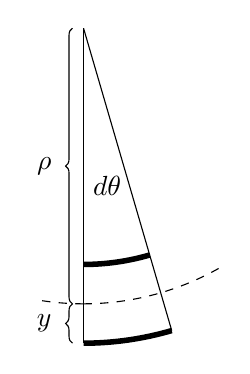
\begin{tikzpicture}
        \draw[-] (0, 0)--(0, -4);
        \draw[-] (0, 0)--(1.12, -3.84);
        \draw[line width=2pt] (0, -4)arc(-90: -73.74: 4);
        \draw[line width=2pt] (0, -3)arc(-90: -73.74: 3);
        \draw[dashed] (0, -3.5)arc(-90: -60: 3.5);
        \draw[dashed] (0, -3.5)arc(-90: -100: 3.5);

        \node at (0.3, -2) {$d \theta$};
        \draw[decorate,decoration={brace, mirror, raise=4pt}] (0, 0)--(0, -3.5);
        \node at (-0.5, -1.75) {$\rho$};
        \draw[decorate,decoration={brace, mirror, raise=4pt}] (0, -3.5)--(0, -4);
        \node at (-0.5, -3.75) {$y$};
    \end{tikzpicture}
    \caption{Bending of the beam}
    \label{Bending of the beam}
\end{figure}

In fig.\ref{Bending of the beam} $\rho d\theta=dx$ which means there's no change on neutral layer. 
Thus the strain $\varepsilon(y)$ at position $y$ is:
\begin{equation}
    \begin{aligned}
        \varepsilon(y)&=
        \frac{dl}{dx}\\
        &=
        \frac{(\rho+y)d\theta - \rho d\theta}{\rho d\theta}\\
        &=\frac{y}{\rho}
    \end{aligned}
\end{equation}

By virture of Hooke's law we have the tensor $\sigma(y)$:
\begin{equation}
    \sigma(y) = E\varepsilon(y)=E\frac{y}{\rho}
\end{equation}

The bending moment on the cross section of the beam is equal to the bending moment produced by sum of $\sigma(y)$:
\begin{equation}
    \begin{aligned}
        M&=
        \int_A
        \sigma(y)y
        dA\\
        &=
        \frac{E}{\rho}
        \int_A y^2 dA
    \end{aligned}
\end{equation}

For a circular section it's obvious that:
\begin{equation}
    \int_A y^2 dA = 
    \int_A z^2 dA
\end{equation}

and use integrate in polar coordinates we have:
\begin{equation}
    \begin{aligned}
        \int_A y^2 dA+\int_A z^2 dA
        &=
        \int_A
        R^2
        dA
        \\
        &=\int_0^{2\pi}d\theta
        \int_0^r R^3dR\\
        &=\frac{\pi}{2}r^4\\
        &=
        \frac{\pi}{32}d^4
    \end{aligned}
\end{equation}

Denote $J_z$ be $\int_A y^2 dA$ we will have its value in the case of circular section that:
\begin{equation}
    J_z=J_y = \frac{\pi}{64}d^4
\end{equation}

Thus the relation of distribution over the beam $M(x)$ with $w(x)$ can be written as:
\begin{equation}
    \label{w''}
    \frac{M}{EJ} = \frac{dw^2}{dx^2}
\end{equation}

For the distribution of $F$ and $q$ is the first and second derivative of $M(x)$, 
finally we have the governing equation of the beam:
\begin{equation}
    \frac{d^4w}{dx^4} = \frac{q}{EJ}
\end{equation}

\subsection{Analytical Solution: Classical Mechanics of Materials}

By virture of classical theory of mechanics of materials we will have the analytical solution. 
Superposition principle reveals that the external forces can be applied on this beam system 
separately.

Denote that:
\begin{equation}
    q=200N/m\quad F=1000N\quad M=2000N\cdot m\quad l=0.12m
\end{equation}
and $J_1$ represents the moment of inertia of thet left hand side's beam and $J_2$ for the right hand side. 
Denote the ground reaction force of the right point is $N$. 
The effect of $q,F,M,N$ to this cantilever beam system (hang on by the left side) is to 
make the right side of the beam's displacement $w_r=0$.

Use superposition principle, let's consider the effect of $q$ on the right hand's displacement $w_{r.q}$ without other external force:
\begin{equation}
    w_{r.q}=
    \frac{q l^3}{6EJ_1}\cdot l+
    \frac{q l^4}{8EJ_1}
\end{equation}

where the first part means the angle at the interface of the two beams and the second part means the displacement at the interface. 
Similarly we have $w_{r.F}$:
\begin{equation}
    w_{r.F} = \frac{Fl^2}{2EJ_1}\cdot l + \frac{Fl^3}{3EJ_1}
\end{equation}

and $w_{r.M}$ equals to:
\begin{equation}
    w_{r.M}= 
    \frac{Ml}{EJ_1}\cdot l + \frac{Ml^2}{2EJ_1} + \frac{Ml^2}{2EJ_2}
\end{equation}

where the first and second part represent the displacement caused by a equivalent force system of $M$ to the beam system's left hand. 
Meanwhile the third part represents the $M$'s effect on the right hand of the beam system. 
Similarly we have the $w_{r.N}$ as below:
\begin{equation}
    w_{r.N}=-
    \left[
        \left(
            \frac{Nl^2}{2EJ_1}+
            \frac{(Nl)\cdot l}{EJ_1}
        \right)\cdot l
        +
        \frac{Nl^3}{3EJ_1}
        +
        \frac{(Nl)\cdot l^2}{2EJ_1}
        +
        \frac{Nl^3}{3EJ_2}
    \right]
\end{equation}

The '-' represents that the $N$ is opposite to the direction of $F$ which make the displacement $w_r$ be negative. 
Thus we get the value of $N$:
\begin{equation}
    N=
    \frac{
        7J_2 l^2 q + 
        20J_2 l F +
        (12 J_1+ 36J_2) M
    }{(8J_1 + 56J_2)L}
\end{equation}

Set the origin point $(0, 0)$ at the left side of the beam. 
Let's first calculate the distribution of $M(x)$. 
$M(0)$ is equal to:
\begin{equation}
    \begin{aligned}
        M_0=M(0)&=
        -\frac{1}{2}ql^2-
        Fl-
        2Nl-
        M
    \end{aligned}
\end{equation}

as well as $F(0)$ is equal to:
\begin{equation}
    F_0=F(0)=
    ql+F - N
\end{equation}

Thus the distribution of $M(x)$ over the beam is:
\begin{equation}
    M(x)=
    \begin{cases}
        \begin{aligned}
            &
            -\frac{1}{2}qx^2 + F_0 x + M_0\quad 0< x < l\\
            &
            -ql\left(
                x-l+\frac{l}{2}
            \right)
            -F(x-l)
            +F_0 x
            +M_0\quad l\leq x < 2l
        \end{aligned}
    \end{cases}
\end{equation}

Denote $EJ(x)$ as:
\begin{equation}
    EJ(x)=
    \begin{cases}
        \begin{aligned}
            E_sJ_1&\quad 0< x < l\\
            E_sJ_2&\quad l< x < 2l
        \end{aligned}
    \end{cases}
\end{equation}

use eq.\ref{w''} we will have the analytical solution of $\theta(x)$ and $w(x)$. 
For the symbolic equation is complex, I just write down the equation numerically:
\begin{equation}
    \theta(x)=
    \begin{cases}
        \begin{aligned}
            &-0.00419174 x^3-0.999404 x^2+0.243843 x\quad 0\leq x < 0.12\\
            &-5.38543 x^2+1.31177 x-0.0649994\quad 0.12\leq x \leq 0.24
        \end{aligned}
    \end{cases}
\end{equation}

\begin{equation}
    w(x)=
    \begin{cases}
        \begin{aligned}
            &-0.00104793 x^4-0.333135 x^3+0.121922 x^2 \quad 0\leq x < 0.12\\
            &-1.79514 x^3+0.655884 x^2-0.0649994 x+0.00263701 \quad 0.12\leq x \leq 0.24
        \end{aligned}
    \end{cases}
\end{equation}

Draw the analytical solution of $\theta(x)$ and $w(x)$ in fig.\ref{Analytical solution}.

\begin{figure}[H]
    \centering
    \subfloat[analytical solution of $\theta(x)$]{
        \includegraphics[width=0.7\textwidth]{..//problem3/image/analytical_theta.pdf}
    }\\
    \subfloat[analytical solution of $w(x)$]{
        \includegraphics[width=0.7\textwidth]{..//problem3/image/analytical_w.pdf}
    }
    \caption{Analytical solution}
    \label{Analytical solution}
\end{figure}

This part is done by Mathematica, you may found it in directory 'problem3//data//task3\_part1.nb'.

\subsection{FEM Method: Hermite Interpolation}


Consider a 1D element (cell) of which the left node's position is $x_1$ and the right node's position $x_2$, 
denote the length of the cell is $h=x_2-x_1$, which is shown in fig.\ref{Hermite interpolation cell}.

\begin{figure}[H]
    \centering
    \begin{tikzpicture}
        \draw[-](0, 0)--(5, 0);
        \draw[-](0, 0)--(0, 0.3);
        \draw[-](5, 0)--(5, 0.3);
        \node at (0, -0.3) {$x_1$};
        \node at (5, -0.3) {$x_2$};
        \node at (2.5, -0.5) {$h$};

        \node at (0, 0.6) {$u_1$};
        \node at (0, 1.2) {$u_1^\prime$};
        \node at (5, 0.6) {$u_2$};
        \node at (5, 1.2) {$u_2^\prime$};
    \end{tikzpicture}
    \caption{Hermite interpolation cell}
    \label{Hermite interpolation cell}
\end{figure}

Assuming that a distribution of parameter $u$ over the cell $u(x)$ satisfies a cubic function:
\begin{equation}
    u(x)=a_0+a_1x+a_2x^2+a_3x^3
\end{equation}

Assume $u(x)$ at the boundary is $u_1$ and $u_2$, as well as $\frac{du(x)}{dx}$'s value $u_1^\prime, u_2^\prime$. 
Thus we have:
\begin{equation}
    \begin{bmatrix}
        1&x_1&x_1^2&x_1^3\\
        0&1&2x_1&3x_1^2\\
        1&x_2&x_2^2&x_2^3\\
        0&1&2x_2&3x_2^2
    \end{bmatrix}
    \begin{bmatrix}
        a_0\\a_1\\a_2\\a_3
    \end{bmatrix}
    =
    \begin{bmatrix}
        u_1\\u_1^\prime\\u_2\\u_2^\prime
    \end{bmatrix}
\end{equation}

Thus $u(x)$ can be written as:
\begin{equation}
    u(x)=
    \begin{bmatrix}
        1&x&x^2&x^3
    \end{bmatrix}
    \begin{bmatrix}
        1&x_1&x_1^2&x_1^3\\
        0&1&2x_1&3x_1^2\\
        1&x_2&x_2^2&x_2^3\\
        0&1&2x_2&3x_2^2
    \end{bmatrix}^{-1}
    \begin{bmatrix}
        u_1\\u_1^\prime\\u_2\\u_2^\prime
    \end{bmatrix}
\end{equation}

Denote that:
\begin{equation}
    \begin{bmatrix}
        \phi_{10}(x)&
        \phi_{11}(x)&
        \phi_{20}(x)&
        \phi_{21}(x)
    \end{bmatrix}=
    \begin{bmatrix}
        1&x&x^2&x^3
    \end{bmatrix}
    \begin{bmatrix}
        1&x_1&x_1^2&x_1^3\\
        0&1&2x_1&3x_1^2\\
        1&x_2&x_2^2&x_2^3\\
        0&1&2x_2&3x_2^2
    \end{bmatrix}^{-1}
\end{equation}

thus the $u(x)$ can be written as a linear combination of the value on the node. 
For convenience, denote:
\begin{equation}
    \begin{aligned}
        \mu_1=u_1\quad
    \mu_2=u_1^\prime\quad
    &
    \mu_3=u_2\quad
    \mu_4=u_2^\prime\\
    \phi_1(x)=\phi_{10}(x)\quad
    \phi_2(x)=\phi_{11}(x)\quad
    &
    \phi_3(x)=\phi_{20}(x)\quad
    \phi_4(x)=\phi_{10}(x)\quad
    \end{aligned}
\end{equation}

thus:
\begin{equation}
    u(x)=
    \sum_{j=1}^4
    \phi_j(x)\mu_j
\end{equation}

The governing equation is given as:
\begin{equation}
    Au=f
\end{equation}

use galerkin method we will have:
\begin{equation}
    \label{Au-f}
    \int_{x_1}^{x_2}
    (Au-f)\phi_i(x)
    dx=0
    \quad i=1,2,3,4
\end{equation}

In the beam's case, governing equation is:
\begin{equation}
    \frac{d^4w(x)}{dx^4}=
    \frac{q(x)}{EJ(x)}=f(x)
\end{equation}

From eq.\ref{Au-f} we have:
\begin{equation}
    \sum_{j=1}^4
    \mu_j
    \int_{x_1}^{x_2}
    \phi_i\frac{d^4\phi_j}{dx^4}dx
    =
    \int_{x_1}^{x_2}
    f\phi_i
    dx
\end{equation}

use integrate by part we will have:
\begin{equation}
    \begin{aligned}
        \int_{x_1}^{x_2}
        \phi_i\frac{d^4\phi_j}{dx^4}
        dx
        &=
        \left.
        \phi_i\frac{d^3\phi_j}{dx^3}
        \right|_{x_1}^{x_2}
        -
        \int_{x_1}^{x_2}
        \frac{d\phi_i}{dx}\frac{d^3\phi_j}{dx^3}
        dx\\
        &=
        \left.
        \phi_i\frac{d^3\phi_j}{dx^3}
        \right|_{x_1}^{x_2}
        -
        \left.
        \frac{d\phi_i}{dx}\frac{d^2\phi_j}{dx^2}    
        \right|_{x_1}^{x_2}
        +
        \int_{x_1}^{x_2}
        \frac{d^2\phi_i}{dx^2}
        \frac{d^2\phi_j}{dx^2}
        dx
    \end{aligned}
\end{equation}

neglect the part $\left.H(\phi_i,\phi_j)\right|_{x_1}^{x_2}$ we will have:
\begin{equation}
    \sum_{j=1}^4
    \mu_j
    \int_{x_1}^{x_2}
    \frac{d^2\phi_i}{dx^2}
    \frac{d^2\phi_j}{dx^2}
    dx
    =
    \int_{x_1}^{x_2}
    f\phi_i
    dx
\end{equation}

In the beam's case we have:
\begin{equation}
\begin{bmatrix}
 \frac{12}{h^3} & \frac{6}{h^2} & -\frac{12}{h^3} & \frac{6}{h^2} \\
 \frac{6}{h^2} & \frac{4}{h} & -\frac{6}{h^2} & \frac{2}{h} \\
 -\frac{12}{h^3} & -\frac{6}{h^2} & \frac{12}{h^3} & -\frac{6}{h^2} \\
 \frac{6}{h^2} & \frac{2}{h} & -\frac{6}{h^2} & \frac{4}{h} \\
\end{bmatrix}
\begin{bmatrix}
    w_1\\ \theta_1\\ w_2\\ \theta_2
\end{bmatrix}
=
\begin{bmatrix}
    \int_{x_1}^{x_2} \frac{q}{EJ}\phi_1 dx\\
    \int_{x_1}^{x_2} \frac{q}{EJ}\phi_2 dx\\
    \int_{x_1}^{x_2} \frac{q}{EJ}\phi_3 dx\\
    \int_{x_1}^{x_2} \frac{q}{EJ}\phi_4 dx
\end{bmatrix}
\end{equation}

Here, if $\frac{q}{EJ}$ is constant, we will have:
\begin{equation}
    \begin{bmatrix}
        \frac{12}{h^3} & \frac{6}{h^2} & -\frac{12}{h^3} & \frac{6}{h^2} \\
        \frac{6}{h^2} & \frac{4}{h} & -\frac{6}{h^2} & \frac{2}{h} \\
        -\frac{12}{h^3} & -\frac{6}{h^2} & \frac{12}{h^3} & -\frac{6}{h^2} \\
        \frac{6}{h^2} & \frac{2}{h} & -\frac{6}{h^2} & \frac{4}{h} \\
       \end{bmatrix}
       \begin{bmatrix}
           w_1\\ \theta_1\\ w_2\\ \theta_2
       \end{bmatrix}
       =
       \frac{q}{EJ}
       \begin{bmatrix}
       \frac{h}{2}\\
       \frac{h^2}{12}\\
       \frac{h}{2}\\
       -\frac{h^2}{12}
       \end{bmatrix}
\end{equation}

If there's only a concentrated load $F_{ex}$ at $x_2$ on this cell, which prescribed that:
\begin{equation}
    \lim_{\varepsilon\to0}
    \left[
        F(x_2) - F(x_2-\varepsilon)
    \right]
    =F_{ex}
\end{equation}

denote that $F_1=F(x_1),F_2=F(x_2)$, obviously that:
\begin{equation}
    F(x)=
    \begin{cases}
        \begin{aligned}
            &F_1 \quad x_1\leq x < x_2\\
            &F_2=F_1 + F_{ex} \quad x=x_2
        \end{aligned}
    \end{cases}
\end{equation}

we can calculate that:
\begin{equation}
    \begin{aligned}
        \int_{x_1}^{x_2}
        \frac{q}{EJ}\phi_i
        dx
        &=
        \left.
        \frac{F}{EJ}\phi_i
        \right|_{x_1}^{x_2}-
        \int_{x_1}^{x_2}
        \frac{F}{EJ}\frac{d\phi_i}{dx}
        dx\\
        &=
        \frac{F_2}{EJ}
        \begin{bmatrix}
            0\\0\\1\\1
        \end{bmatrix}
        -
        \frac{F_1}{EJ}
        \begin{bmatrix}
            1\\1\\0\\0
        \end{bmatrix}
        -\frac{F_1}{EJ}
        \begin{bmatrix}
            -1\\0\\1\\0
        \end{bmatrix}\\
        &=
        \frac{1}{EJ}
        \begin{bmatrix}
            0\\
            -F_1\\
            F_{ex}\\
            F_2
        \end{bmatrix}
    \end{aligned}
\end{equation}

For $F_1,F_2$ will be compensated by the cell's neighbourhood, this part can be written as:
\begin{equation}
    \int_{x_1}^{x_2}
        \frac{q}{EJ}\phi_i
        dx
        =
        \frac{1}{EJ}
        \begin{bmatrix}
            0\\
            0\\
            F_{ex}\\
            0
        \end{bmatrix}
\end{equation}

Similarly, suppose we only have a concentrated bending moment $M_{ex}$ at $x_2$ and use the same symbolic mark:

\begin{equation}
    M(x)=
    \begin{cases}
        \begin{aligned}
            &M_1 \quad x_1\leq x < x_2\\
            &M_2=M_1 + M_{ex} \quad x=x_2
        \end{aligned}
    \end{cases}
\end{equation}

thus:
\begin{equation}
    \begin{aligned}
        \int_{x_1}^{x_2}
        \frac{q}{EJ}\phi_i
        dx
        &=
        \left.
        \frac{F}{EJ}\phi_i
        \right|_{x_1}^{x_2}-
        \int_{x_1}^{x_2}
        \frac{F}{EJ}\frac{d\phi_i}{dx}
        dx\\
        &=
        \left.
        \frac{F}{EJ}\phi_i
        \right|_{x_1}^{x_2}
        -
        \left.
        \frac{M}{EJ}\frac{d\phi_i}{dx}
        \right|_{x_1}^{x_2}
        +
        \int_{x_1}^{x_2}
        \frac{M}{EJ}\frac{d^2\phi_i}{dx^2}
        dx\\
        &=
        \frac{M_1}{EJ}
        \begin{bmatrix}
            0\\-1\\0\\1
        \end{bmatrix}
        -
        \frac{M_2}{EJ}
        \begin{bmatrix}
            0\\0\\0\\1
        \end{bmatrix}
        +
        \frac{M_1}{EJ}
        \begin{bmatrix}
            0\\1\\0\\0
        \end{bmatrix}\\
        &=
        \frac{1}{EJ}
        \begin{bmatrix}
            0\\
            0\\
            0\\
            -M_{ex}
        \end{bmatrix}
    \end{aligned}
\end{equation}

To conclude, 
we have the relation on this cell part as the format $[K]u=b$:
\begin{equation}
    EJ
    \begin{bmatrix}
        \frac{12}{h^3} & \frac{6}{h^2} & -\frac{12}{h^3} & \frac{6}{h^2} \\
        \frac{6}{h^2} & \frac{4}{h} & -\frac{6}{h^2} & \frac{2}{h} \\
        -\frac{12}{h^3} & -\frac{6}{h^2} & \frac{12}{h^3} & -\frac{6}{h^2} \\
        \frac{6}{h^2} & \frac{2}{h} & -\frac{6}{h^2} & \frac{4}{h} \\
       \end{bmatrix}
       \begin{bmatrix}
           w_1\\ \theta_1\\ w_2\\ \theta_2
       \end{bmatrix}
       =
       q_{ex}
       \begin{bmatrix}
        \frac{h}{2}\\
        \frac{h^2}{12}\\
        \frac{h}{2}\\
        -\frac{h^2}{12}
        \end{bmatrix}
        +
        \begin{bmatrix}
            0\\
            0\\
            F_{ex}\\
            -M_{ex}
        \end{bmatrix}
\end{equation}

And the application of $q_{ex}, F_{ex}, M_{ex}$ is shown in fig.\ref{Bernoulli-Euler beam element}.

\begin{figure}[H]
    \centering
    \begin{tikzpicture}
        \draw[-](0, 0)--(5, 0);
        \draw[-](0, 0)--(0, 0.3);
        \draw[-](5, 0)--(5, 0.3);
        \node at (0, -0.3) {$x_1$};
        \node at (5, -0.3) {$x_2$};
        \node at (2.5, -0.5) {$h$};

        \draw[->] (5, -3)--(5, -2);
        \node at (5, -3.3) {$F_{ex}$};

        \node at (0, 0.6) {$w_1$};
        \node at (0, 1.2) {$\theta_1$};
        \node at (5, 0.6) {$w_2$};
        \node at (5, 1.2) {$\theta_2$};

        \draw[<->] (5.1, -1)--(5.5, -1)--(5.5, 1)--(5.9, 1);
        \node at (5.9, 0) {$M_{ex}$};

        \draw[-] (0, -1.5)--(5, -1.5);
        \foreach \i in {0,0.5,1,...,5}{
            \draw[->] (\i, -1.5) -- (\i, -1);
        };
        \node at (2.5, -2) {$q_{ex}$};
    \end{tikzpicture}
    \caption{Bernoulli-Euler beam element}
    \label{Bernoulli-Euler beam element}
\end{figure}

You may find all these formula derivation progress in 'problem3/data/task3\_part2.nb' Mathematica notebook. 
In case you have no Mathematica on your computer, I print this file as 'task3\_part2.pdf' in which the detailed derivation is included.



\subsection{Programming: Julia Code}

For convenience, uniform 1-D mesh is considered. 
Also I choose Julia to finish this project. 
You may find my codes under directory 'problem3/src/'. 
Here's a brief description of the julia codes.

\begin{enumerate}
    \item Case.jl: to set a case for this calculation. There's one struct and two functions in it:
    \begin{itemize}
        \item Case: struct, use to store the calculation parameters;
        \item moment\_of\_inertia: function, calculate the moment of inertia on circular section when diameter $d$ is given;
        \item Case: function, to generate a default Case struct. It is noteworthy that to show the advance of Hermite interpolation, I choose to devide the beam into only $\text{devide}=10$ cells on each side.
    \end{itemize}
    \item HermiteFEM.jl: to solve the problem including:
    \begin{itemize}
        \item generate\_K\_b: function, to generate ths $[K]u=b$ 's $[K]$ and $b$ from the case;
        \item solve: function, to solve the given case;
        \item hermite\_interpolation: function, to generate a interpolation function from the calculation result;
        \item interpolation\_minor: function, refine the value inside the cells. Here 'default\_minor=4' which means there will be 4 more nodes' values on each cell generated by Hermite interpolation.
    \end{itemize}
    \item Main.jl: the main code to solve the case and draw the picture.
\end{enumerate}

\subsection{Julia Code Result: Hermite Interpolation inside the Cell}

Denote that cell $k$ at position $[x_k,x_{k+1}]$, and $t = x-x_1, h=x_2-x_1$. 
We will have the $w(x),\theta(x)$ 's value inside the cell:
\begin{equation}
    w(x)=
    \frac{(h-t^2)(h+2t)}{h^3}w_{k}+
    \frac{t(h-t)^2}{h^2}\theta_{k}+
    \frac{t^2(3h-2t)}{h^3}w_{k+1}+
    \frac{t^2(t-h)}{h^2}\theta_{k+1}\quad
    x_1\leq x < x_2
\end{equation}

\begin{equation}
    \theta(x)=
    \frac{6t(t-h)}{h^3}w_{k}+
    \frac{(h-3t)(h-t)}{h^2}\theta_{k}+
    \frac{6t(h-t)}{h^3}w_{k+1}+
    \frac{t(3t-2h)}{h^2}\theta_{k+1}\quad
    x_1\leq x < x_2
\end{equation}

Such derivation is also included in file 'problem3//data//task3\_part2.nb' Mathematica notebook.

Within Julia code, I separate the 1-D domain into $21$ nodes and $20$ cells, 
in which $10$ for the left side's beam and $10$ for the right side's beam. 
By virture of package 'SparseArrays.jl', it's possible to devide the domain into large cells. 
I've tested the case of $10001$ nodes and the total run time of solution is only 0.24 seconds on my 8th Intel CPU 8750H. 
However, to show the advance of Bernoulli-Euler beam elements, only $21$ nodes are given. 
You may change the number of nodes by modify the value 'devide' in given struct case.

Fig.\ref{Julia code solution} shows the julia code solution, of which 
the red points are the interpolation nodes and the blue curve is generated by inner hermite interpolation.

\begin{figure}[H]
    \centering
    \subfloat[julia code solution of $\theta(x)$]{
        \includegraphics[width=0.7\textwidth]{..//problem3/image/julia_theta.pdf}
    }\\
    \subfloat[julia code solution of $w(x)$]{
        \includegraphics[width=0.7\textwidth]{..//problem3/image/julia_w.pdf}
    }
    \caption{Julia code solution}
    \label{Julia code solution}
\end{figure}

\subsection{Validation: Comparison with Analytical Solution}

Draw the analytical curve and julia FEM method code's curve in the same figure, 
we will have the comparison in fig.\ref{Comparison with analytical solution}.

\begin{figure}[H]
    \centering
    \subfloat[julia code solution of $\theta(x)$]{
        \includegraphics[width=0.7\textwidth]{..//problem3/image/comparison_theta.pdf}
    }\\
    \subfloat[julia code solution of $w(x)$]{
        \includegraphics[width=0.7\textwidth]{..//problem3/image/comparison_w.pdf}
    }
    \caption{Comparison with analytical solution}
    \label{Comparison with analytical solution}
\end{figure}